% !TeX root = RJwrapper.tex
\title{pksensi: A Package to Apply Global Sensitivity Analysis in
Physiologically Based Kinetic Modeling}
\author{by Nan-Hung Hsieh, Brad Reisfeld, Weihsueh A. Chiu}

\maketitle

\abstract{%
We developed a package, named \CRANpkg{pksensi}, to make global
sensitivity analysis (SA) more accessible in physiologically based
kinetic modeling. This package can investigate both parameter
uncertainty and sensitivity in pharmacokinetic models, including those
with multivariate model outputs, such as multiple time-points and tissue
compartments. We refined the extended Fourier Amplitude Sensitivity Test
method for SA by adding a random phase-shift to analyze the statistical
variability of the sensitivity index for each model parameter.
Furthermore, it includes functions to check the convergence of the
global SA results. Utilizing \CRANpkg{pksensi}, we successfully
reproduced our previously published SA results of human physiologically
based pharmacokinetic modeling for acetaminophen and its two primary
metabolites. Overall, \CRANpkg{pksensi} improves the user experience of
performing global SA and can create robust and reproducible results for
decision making in pharmacokinetic model calibration.
}


\hypertarget{introduction}{%
\section{Introduction}\label{introduction}}

Sensitivity analysis (SA) is a mathematical technique to investigate how
variations in model parameters affect model outputs. An increasing
number of studies use SA to determine which model parameters contribute
to high variation in model predictions \citep{ferretti2016trends}. This
technique has also been applied in pharmacology and toxicology research
\citep{loizou2015application, mcnally2012reconstruction}.
Pharmacokinetic (PK) models describe the changes in the concentrations
or amounts of a substance in the body over time (the various terms for
the kinetic models, including ``pharmacokinetic'', ``toxicokinetic'',
and ``biokinetic'' models, are used exchangeably here). The goal of SA
in PK research is to examine the sensitivity of output variables, such
as chemical concentration in blood or tissues, with respect to input
parameters, such as anatomical, physiological, and kinetic constants
\citep{mcnally2011workflow}. In addition, this SA approach can guide
experimental design and the parameter estimation processes
\citep{zhang2015sobol}. For instance, SA can identify ``unidentifiable''
parameters that can lead to problems with numerical procedures used in
parameter estimation \citep{chu2010quantitative}. It can be further
applied to parameter prioritization and parameter fixing before model
calibration \citep{fphar201800588}.

In our earlier work \citep{fphar201800588}, we developed an updated
workflow to apply global SA to reduce the computational burden in the
Bayesian, Markov Chain Monte Carlo (MCMC)-based calibration process of a
physiologically based pharmacokinetic (PBPK) model. We used GNU MCSim
\citep{bois2009gnu}, an effective simulation package for Bayesian
population PBPK modeling, to calibrate the model. We found that the
extended Fourier Amplitude Sensitivity Test (eFAST), a type of
variance-based global SA algorithm, had the best balance of efficiency
and accuracy for a sophisticated, multi-compartment, multi-dataset, and
multi-metabolite PBPK model. This method was first introduced in
\citet{cukier1973study} (the classic FAST method with the first-order
effect only) in a study of the sensitivity of coupled reaction systems
that are constructed by differential equations with the numerous rate
coefficients. It then evolved to estimate the Sobol' sensitivity measure
in \citet{saltelli1999quantitative} (the eFAST method with first- and
total-order effects). The FAST algorithm creates the multidimensional
space of input parameters through a ``search-curve''. It is more
computationally efficient in calculating the influence of model
parameter than other global SA methods such as the Monte Carlo based
approaches \citep{jansen1999analysis, owen2013better}. Our previous work
also found some efficient visualization approaches that can be used to
distinguish between ``influential'' and ``non-influential'' parameters.
This approach addresses common identifiability issues of PBPK model
parameter that increase the computational burden of Bayesian analysis
\citep{garcia2015identifiability}, and therefore reduce the
computational efficiency. We also developed approaches for communicating
parameter sensitivity in decision making.

There are numerous developed packages, such as \CRANpkg{sensitivity}
\citep{R-sensitivity}, which is a practical tool to conduct local and
global SA. The \CRANpkg{sensitivity} package includes some functions to
generate the parameter sequences by using different computing
algorithms. Also, it provides a feasible way to integrate external
modeling results. This computational approach can effectively solve the
heavy computing burden of numerical solutions within the pure R
environment. Several other R packages, such as \CRANpkg{FME},
\CRANpkg{multisensi}, and \CRANpkg{ODEsensitivity} include SA tools and
are freely available in the Comprehensive R Archive Network (CRAN). The
\CRANpkg{FME} package contains a basic method for performing local SA
for dynamic models \citep{JSSv033i03}. It can also conduct collinearity
and identifiability analysis to evaluate which model parameters can
estimate or exclude based on available observation data. The
\CRANpkg{multisensi} package provides SA for models with multivariate
output \citep{R-multisensi}. \CRANpkg{ODEsensitivity} can perform SA in
ordinary differential equation (ODE) models \citep{R-ODEsensitivity}. It
utilizes the ODE interface from the \CRANpkg{deSolve} package and
connect it with the SA from the \CRANpkg{sensitivity} package. Other
related packages such as \CRANpkg{mtk} \citep{RJ-2015-031} and
\CRANpkg{fast} \citep{R-fast} are designed to investigate the importance
of model parameter.

Although these tools provide various approaches to perform SA, they each
individually have limitations for application to PK modeling. For
example, the estimated index in SA is not robust when using the
inadequate size of the sample number. However, there are no software
packages that provide the available tools in the assessment of
reliability. In addition, the existing eFAST function does not include
the feature to generate the random sampling curve. We present here an
package, called \CRANpkg{pksensi}, which is designed to make SA more
accessible and reproducible in pharmacological and toxicological
researches. This package can investigate both parameter uncertainty and
sensitivity in PK model with multivariate model outputs. Moreover, it
seamlessly integrates with both general ODE solvers available in R or as
external C code, as well as the GNU MCSim software used for conducting
sophisticated PK modeling, including MCMC. The analytical framework in
\CRANpkg{pksensi} includes not only global SA but also the uncertainty
analysis and diagnostic tools to support the modeling process.

\hypertarget{workflow}{%
\section{Workflow}\label{workflow}}

\hypertarget{installation}{%
\subsection{Installation}\label{installation}}

The \CRANpkg{pksensi} package can link with \CRANpkg{deSolve} package,
which includes a comprehensive integrator to solve ODE. The GNU MCSim
can be installed by following the instruction in GNU MCSim's manual on
\url{https://www.gnu.org/software/mcsim/mcsim.html} or using the
built-in function \code{mcsim\_install} in \CRANpkg{pksensi}. The C
compiler is already available in Linux or MacOS. The Windows user can
install Rtools and set the working path of compiler before using this
function as:

\begin{Schunk}
\begin{Sinput}
Rtools.path <- "c:/Rtools/bin; c:/Rtools/mingw_64/bin"
Sys.setenv(PATH = paste(Rtools.path, Sys.getenv("PATH"), sep=";"))
\end{Sinput}
\end{Schunk}

\hypertarget{parameter-matrix-generation}{%
\subsection{Parameter matrix
generation}\label{parameter-matrix-generation}}

We adopted eFAST, the widely used analysis of variance (ANOVA)-like
global SA approach to decompose the variance to partial variances for
multidimensional parameters in numerical models in this package. Most of
the available eFAST functions, such as the algorithm to generate the
parameter space and to set the sampling frequency, were sourced from the
\CRANpkg{sensitivity} package \citep{R-sensitivity}. The eFAST method
computes the sensitivity index (SI) via ANOVA-like decomposition of the
function for analysis. This type of global SA approach and SI also know
as Sobol' method and Sobol' index. Since the estimated SI is not stable
(high variation) when using smaller sample size, we included a random
phase-shift approach to conduct replicating sampling from random
starting points across parameter space to test the convergence and
robustness of the sensitivity measurement. Considering the model that is
built under \(y=f(x_{i})\). The sampling scheme can describe as,

\[ x_i = \frac{1}{2} + \frac{1}{\pi}\arcsin(\sin(\omega_is + \varphi_i)) \]

where \(x_i\) is the nominal value of the \(i\)-th parameter, and
\(\omega_i\) is a vector giving the set of frequencies, one frequency
for each parameter, and \(\varphi\) is a random phase-shift coefficient
ranged from 0 to \(2\pi\). The default set of frequencies is according
to the study from \citet{saltelli1999quantitative}. Through the random
phase-shift, the robust result of the sensitivity measurement should be
similar across each replication under the same sample size. For most
Sobol'-based SA algorithms, the larger sample size is needed to reduce
the probability of having negative estimates. However, FAST estimates
are always positive according to its construction.

To investigate the convergence of SI, we adopted the ``exam'' approach
proposed by \citep{sarrazin2016global}. This method quantitatively
assesses convergence by computing the width of 95\% confidence intervals
of computed SI for all parameters across all time-points and output
variables. Through random phase-shift procedure, the replicated SI
values can repeatedly sample independently. Therefore, they can be used
to investigate the convergence of SI as,

\[CI_{i,t} = max(SI_{i,t}^{ub}-SI_{i,t}^{lb})\]

where \(SI_{i,t}^{ub}\) and \(SI_{i,t}^{ub}\) are the upper and lower
bound of the SI from the specific model output (\(i\)) at time (\(t\)).
\(CI_{i,t}\) is the corresponding convergence index.

To integrate the random phase-shift with eFAST, we built the
\code{rfast99} function, which can be used to perform the sensitivity
test for the whole modeling process. The function \code{rfast99} in
\CRANpkg{pksensi} can sample and generate the testing parameter matrix
based on a given argument of sample size \(n\) and probability
distribution (e.g., mean/s.d. of normal distribution, meanlog/sdlog of
log-normal distribution, and minimum/maximum of uniform distribution).
The number of model evaluations is equal to the sample size times the
number of model parameters.

\hypertarget{modeling}{%
\subsection{Modeling}\label{modeling}}

The \CRANpkg{pksensi} package provides a useful function to solve ODEs
in PK models using analytical and numerical approaches. The solution can
perform under the pure R programming environment by linking
\CRANpkg{pksensi} with the \CRANpkg{deSolve} package \citep{JSSv033i09}.
However, the most efficient way to achieve high computational speed is
through compiled, lower-level languages, such as FORTRAN, C, or C++. The
\CRANpkg{pksensi} package includes a function to compile and create
dynamic-link libraries (.dll) on Windows and shared objects (.so) on
Unix-liked systems (e.g., Linux and MacOS). This compiled program can
load and execute through the build-in function in R. However, Windows
users need to install Rtools to compile the source code by using the GNU
GCC compiler. The C implementation of the example model can be found as
an example within GNU MCSim \citep{bois2009gnu}. The \CRANpkg{pksensi}
can also link with GNU MCSim to create the model program, used in
solving each system of equations.

The uncertainty analysis is a crucial modeling process within SA.
Sometimes, it is difficult to have informative data to set up the
parameter distribution. A wider range for a parameter distribution might
cause a numerical error at extreme values. On the other hand, narrower
ranges might cause the incorrect calibrated result of the model
parameter. The uncertainty analysis using Monte Carlo is an appropriate
approach in the data-driven modeling process to address this problem.
Before fitting the data to model, the Monte Carlo can be applied with
the given distribution of model parameter to examine whether the
experimental data are within the range of the distribution of model
output. \CRANpkg{pksensi} also has a function that can link to GNU MCSim
to conduct Monte Carlo analysis, which is built-into GNU MCSim and
examine the simulation result. The general workflow of uncertainty and
SA is illustrated in Figure \ref{fig:Workflow}.

\begin{Schunk}
\begin{figure}
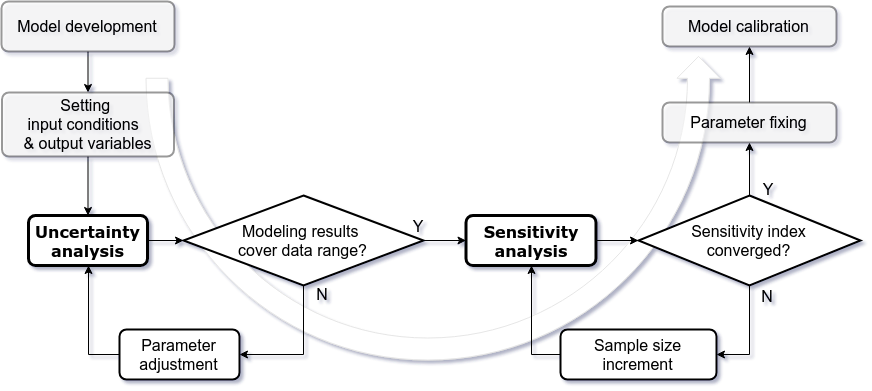
\includegraphics[width=1\linewidth]{diagram/Workflow} \caption{\label{fig:Workflow}Workflow for performing uncertainty and sensitivity analysis.}\label{fig:workflow}
\end{figure}
\end{Schunk}

\hypertarget{output-visualization-and-decision-support}{%
\subsection{Output visualization and decision
support}\label{output-visualization-and-decision-support}}

The output of SA returns a list that contains the given time-points and
values of all state variables (e.g., chemical concentrations in blood).
This format is particularly suited for further graphical routines within
\CRANpkg{pksensi}. Also, time-dependent sensitivity measurements of
first and total effects for all parameters can be plotted
simultaneously. If the computed SI show different values across
replications under the same sample size, this indicates an inadequate
sample number, which can create an unreliable result. It is essential to
use a sufficient sample size to prevent incorrect judgments in parameter
fixing. \CRANpkg{pksensi} includes functions to check the convergence
and sensitivity of model parameters, providing a means to assess the
robustness of the sensitivity measurement. We also developed a
``cut-off''-based approach in this package to distinguish between
``influential'' and ``non-influential'' parameters. Finally,
\CRANpkg{pksensi} provides visualization tools for the effective
investigation and communication of results in decision support.

\hypertarget{example-1-one-compartment-model}{%
\section{Example 1: One-compartment
model}\label{example-1-one-compartment-model}}

In the following section, two PK models will apply to demonstrate how
\CRANpkg{pksensi} works. The first one is a generic model, and the
second is a chemical-specific model.

\hypertarget{equations}{%
\subsection{Equations}\label{equations}}

In the first example, we use a generic, one-compartment PK model from
\CRANpkg{httk} package \citep{JSSv079i04} to demonstrate how
\CRANpkg{pksensi} can apply to PK studies. The differential equations
for this model is as,

\[\frac{dA_{gutlumen}}{dt} = -k_{gutabs} \cdot A_{gutlumen} + g(t)\]
\[\frac{dA_{rest}}{dt} = k_{gutabs} \cdot A_{gutlumen}-k_{elim} \cdot A_{rest}\]

where \(A_{gutlumen}\) is the state variable that describes the quantity
of compound in the gut lumen (mg) and \(A_{rest}\) is the quantity of
compound in rest of body and blood (mg). The parameter \(k_{gutabs}\) is
the absorption rate constant that describes the chemical absorption from
the gut lumen into gut tissue through first-order processes (/h) and
\(k_{elim}\) is the elimination rate constant (/h), which is equal to
the total clearance divided by the volume of distribution. The
time-dependent function \(g(t)\) is used to describe the oral dosing
schedule.

The concentration of the chemical in the rest of body and blood
(\(C_{rest}\), mg/L) can calculate as,

\[ C_{rest} = A_{rest} / V_{dist} \cdot BW\]

where \(V_{dist}\) is the volume of distribution (L/kg BW) and \(BW\) is
the body weight (kg). \(C_{rest}\) can also represent as the chemical
concentration in plasma that can be further used to compare with
observed results in a PK experiment. The bioavailability is assumed to
be 100\% in this model.

\hypertarget{model-implementations-with-desolve-package}{%
\subsection{\texorpdfstring{Model implementations with \textbf{deSolve}
package}{Model implementations with deSolve package}}\label{model-implementations-with-desolve-package}}

To start, we implemented the one-compartment PK model in R. The
\CRANpkg{pksensi} allows users select the preferred method to solve the
PK model, either with the \CRANpkg{deSolve} package or with GNU MCSim
through the compile function. This section mainly focuses on how to
conduct global SA with \CRANpkg{deSolve} package with pure R
environment.

The one-compartment PK model can describe the quantity of compound in
the gut lumen (\code{Agutlument}) and the rest of body
(\code{Acompartmant}). The \code{Ametabolized} is the quantity of
compound transform and metabolize through hepatic clearance.

\begin{Schunk}
\begin{Sinput}
pbtk1cpt <- function(t, state, parameters) {
  with(as.list(c(state, parameters)), {
    dAgutlument = - kgutabs * Agutlument
    dAcompartment = kgutabs * Agutlument - ke * Acompartment
    dAmetabolized = ke * Acompartment
    Ccompartment = Acompartment / vdist * BW;
    list(c(dAgutlument, dAcompartment, dAmetabolized), 
         "Ccompartment" = Ccompartment) 
  })
}
\end{Sinput}
\end{Schunk}

The parameter values and initial states need to be assigned to specific
values before simulation. Here, we use the corresponding parameter value
of acetaminophen (APAP) in this example. These model parameters are
derived from the \emph{in-vivo} or \emph{in-vitro} experiment results.
The parameter value can be generated from \code{parameterize\_1comp}
function in \CRANpkg{httk} package as:

\begin{Schunk}
\begin{Sinput}
library(httk)
pars1comp <- (parameterize_1comp(chem.name = "acetaminophen"))
parms <- c(vdist = pars1comp$Vdist, 
           ke = pars1comp$kelim, 
           kgutabs = pars1comp$kgutabs, 
           BW = pars1comp$BW)
initState <- c(Agutlument = 10, Acompartment = 0, Ametabolized = 0)
\end{Sinput}
\end{Schunk}

The given value of \code{vdist}, \code{ke}, and \code{kgutabs} in
\CRANpkg{httk} are 1.1 (L/kg BW), 0.23 (/h), and 2.18 (/h),
respectively. The body weight is assumed to be 70 (kg).

Here shows the given parameter value (\code{parms}) and initial state
condition (\code{initState}) that need to specify in model solving. Both
\code{parms} and \code{initState} are ``numeric variables'' that contain
the value of parameter and initial state condition.

Using the \code{ode} function in \CRANpkg{deSolve} package, we can
visualize the PK profile (Figure \ref{fig:ode-PK}) according to the
given parameter baseline and the time points (\code{t}).

\begin{Schunk}
\begin{Sinput}
library(deSolve)
t <- seq(from = 0.01, to = 24.01, by = 1)
y <- ode(y = initState, times = t, func = pbtk1cpt, parms = parms)
\end{Sinput}
\end{Schunk}

\begin{Schunk}
\begin{Sinput}
par(mar=c(4,2,2,1))
plot(y)
\end{Sinput}
\begin{figure}

{\centering 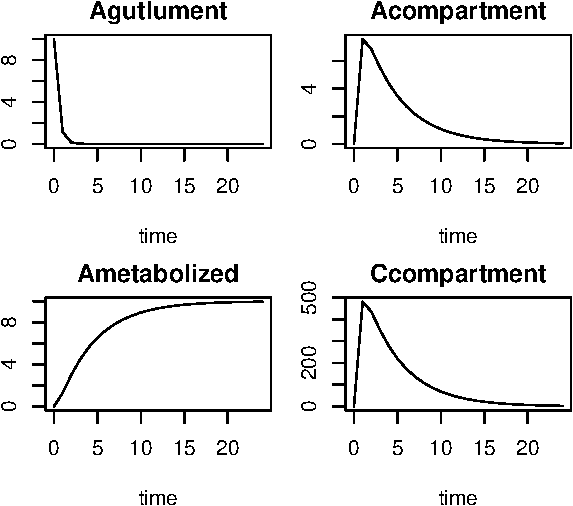
\includegraphics[width=0.6\linewidth]{RJ-pksensi_files/figure-latex/unnamed-chunk-5-1} 

}

\caption{\label{fig:ode-PK}Simulation results of one-compartment PK model for fixed default parameters.}\label{fig:unnamed-chunk-5}
\end{figure}
\end{Schunk}

We conduct global SA for the four parameters in one-compartment PK model
to investigate the parameter impact on the plasma concentration during
the 24-hr time post intake. The distribution of parameter is taken to be
uniform with bounds corresponding to 50\% and 200\% of the nominal
value. Therefore, the parameter ranges are assumed to be 0.55 and 2.2
L/kg BW for \code{vdist}. The \code{ke} are ranged from 0.12 to 0.46 /h,
corresponding to half-times of 1.5 and 5.8 hr. The \code{ka} are ranged
1.09 to 4.36 /h, corresponding to half-times of 0.32 and 0.64 hr. The
\code{BW} is assumed to a normal distribution with mean = 60 kg and sd =
5 kg.

\begin{Schunk}
\begin{Sinput}
q <- c("qunif", "qunif", "qunif", "qnorm")
q.arg <- list(list(min = pars1comp$Vdist / 2, max = pars1comp$Vdist * 2),
              list(min = pars1comp$kelim / 2, max = pars1comp$kelim * 2),
              list(min = pars1comp$kgutabs / 2, max = pars1comp$kgutabs * 2),
              list(mean = pars1comp$BW, sd = 5))
params <- c("vdist", "ke", "kgutabs", "BW")
\end{Sinput}
\end{Schunk}

Here we use a sample size of 200 with 10 replications. Through
\code{rfast99} function, a S3 object with class `rfast99' will be
created. The \code{set.seed} can use to reproduce the same parameter
matrix in the random sampling. The sample size determines the robustness
of the result of SA. Higher number of sample size lead to narrower
confidence intervals for sensitivity measurements across different
replications. However, it will take a longer time in computation.

\begin{Schunk}
\begin{Sinput}
set.seed(1234)
x <- rfast99(params, n = 200, q = q, q.arg = q.arg, replicate = 10)
\end{Sinput}
\end{Schunk}

The generated parameters are stored as a 3-D array under the named
\code{a}, with the dimension of sample size, the number of replications,
and the number of parameters, respectively.

\begin{Schunk}
\begin{Sinput}
dim(x$a)
\end{Sinput}
\begin{Soutput}
  [1] 800  10   4
\end{Soutput}
\end{Schunk}

The sample number is 200, with 4 model parameters, which generates 800
model evaluations. The replication is set to 10. Therefore, the total of
8,000 parameter sequence will be used to compute the corresponding
outputs. Figure \ref{fig:rep-sampl} plotted the sampling process for
each parameter from the first 3 replications. The search curves show the
different intensity of sampling patterns in each segment.

\begin{Schunk}
\begin{Sinput}
par(mfrow=c(4,4),mar=c(0.8,0.8,0.8,0),oma=c(4,4,2,1), pch =".")
for (j in c("vdist", "ke", "kgutabs", "BW")) {
  if ( j == "BW") {
    plot(x$a[,1,j], ylab = "BW")
  } else plot(x$a[,1,j], xaxt="n", ylab = "")
  for (i in 2:3) {
  if ( j == "BW") {
    plot(x$a[,i,j], ylab = "", yaxt="n")  
    } else plot(x$a[,i,j], xaxt="n", yaxt="n", ylab = "")
  } 
  hist <- hist(x$a[,,j], plot=FALSE, 
               breaks=seq(from=min(x$a[,,j]), to=max(x$a[,,j]), length.out=20))
  barplot(hist$density, axes=FALSE, space=0, horiz = T, main = j) 
}
mtext("Model evaluation", SOUTH<-1, line=2, outer=TRUE)
\end{Sinput}
\begin{figure}

{\centering 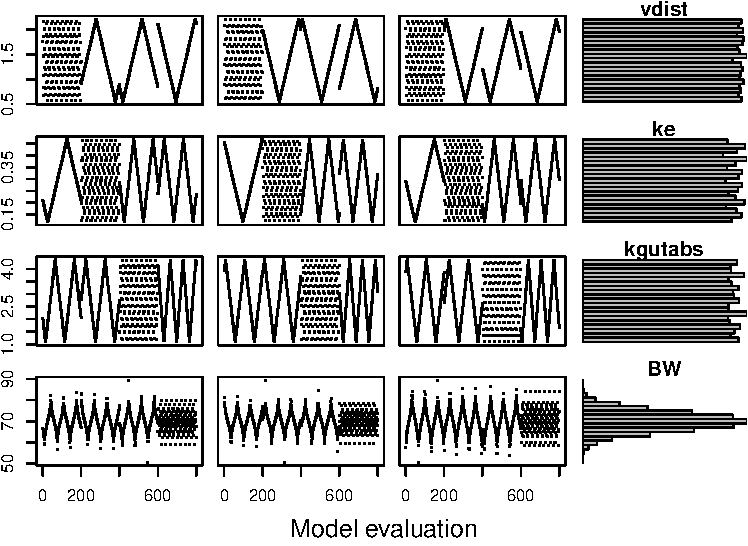
\includegraphics{RJ-pksensi_files/figure-latex/unnamed-chunk-9-1} 

}

\caption{\label{fig:rep-sampl}The parameter search curves generated by eFAST method. The x-axis is the sample number and y-axis is the parameter value for \code{vdist}, \code{ke}, \code{kgutabs}, and \code{BW} (top to down), respectively. The bar plot shows the distribution of sampling parameter.}\label{fig:unnamed-chunk-9}
\end{figure}
\end{Schunk}

Because the PK model is being used to describe a continuous process for
the chemical concentration over time, the sensitivity measurements,
therefore, have the time-dependent relationships for each model
parameter. Here we use the defined output time points (\code{t}) to
examine the change of the parameter sensitivity over time. To solve the
model through \CRANpkg{deSolve}, we need to provide the details of the
argument, which include time (\code{t}), initial conditions of state
variable (\code{initState}), output variables (\code{outnames}), and
name of the model function (\code{func}). To create the time-dependent
sensitivity measurement, we set the time duration from 0.01 to 24.01
hours with the time segment of 1 hour as the above definition in
\code{ode} function in this example. The initial time point should avoid
0 to prevent computational error in misconduct. The \code{outnames} is
based on the arguments from the \code{ode} function in \CRANpkg{deSolve}
package.

\begin{Schunk}
\begin{Sinput}
outputs <- c("Ccompartment", "Ametabolized")
out <- solve_fun(x, time = t, func = pbtk1cpt, 
                 initState = initState, outnames = outputs)
\end{Sinput}
\begin{Soutput}
  Starting time: 2019-10-19 11:26:22
\end{Soutput}
\begin{Soutput}
  Ending time: 2019-10-19 11:27:53
\end{Soutput}
\end{Schunk}

The output result \code{out} is an S3 object of \code{rfast99} as well,
which can link with \code{print}, \code{plot}, and \code{check} method
to examine the sensitivity measurements. The \code{print} function gives
the sensitivity and convergence indices for main, interaction, and total
order at each time point. In addition to print out the result of SA, the
more efficient way to distinguish the influence of model parameter is to
visualize these indices. The time-dependent SI are shown in Figure
\ref{fig:pk-solvefun-rest}. The SI has computed range from 0 (no impact)
to 1 (high impact) and represents the contribution percentage of output
variance under the given parameter distributions.

\begin{Schunk}
\begin{Sinput}
plot(out)
\end{Sinput}
\begin{figure}

{\centering 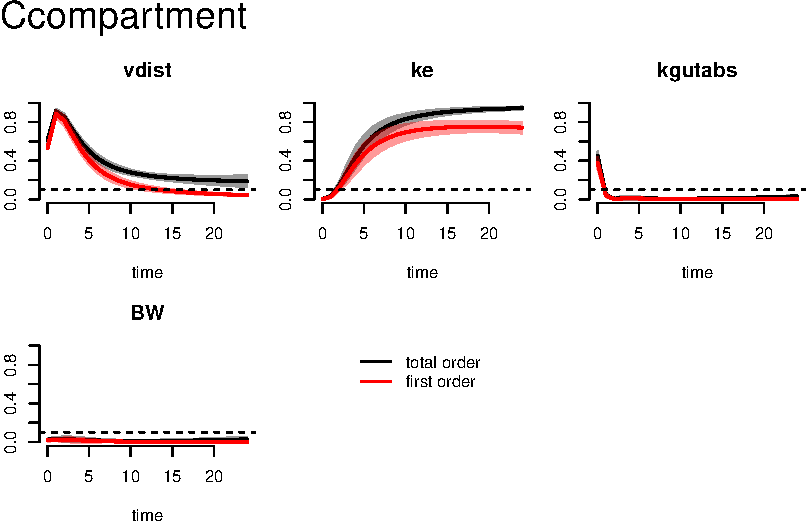
\includegraphics[width=0.8\linewidth]{RJ-pksensi_files/figure-latex/unnamed-chunk-11-1} 

}

\caption{\label{fig:pk-solvefun-rest}Time-dependent SI of the plasma concentration estimated from the one-compartment PK model during 24-hr time period intake. The solid line represents the total (black) and first (red) order SI with 95\% confidence interval (polygon). The dashed line is the cut-off with the default value of 0.05.}\label{fig:unnamed-chunk-11}
\end{figure}
\end{Schunk}

Here, we can see (Figure \ref{fig:pk-solvefun-rest}) that \code{vdist}
and \code{ke} dominate the plasma concentration before and after 5-hr
post chemical intake, respectively. The parameter \code{kgutabs} only
plays a crucial role to determine the plasma concentration in the first
hour. However, the current result only based on the distribution of
model parameters for APAP. Given different input conditions (e.g., range
of parameter uncertainty, chemical-dependent parameter value) the result
can of course change (result not shown).

The default output in the plotting is setting at the first variable. To
exam the time-dependent SI of other variables, such as
\code{Ametabolized} in this case, we need to assign the variable name
\code{vars = "Ametabolized"} in \code{plot} function (Figure
\ref{fig:pk-solvefun-Amet}).

\begin{Schunk}
\begin{Sinput}
plot(out, vars = "Ametabolized")
\end{Sinput}
\begin{figure}

{\centering 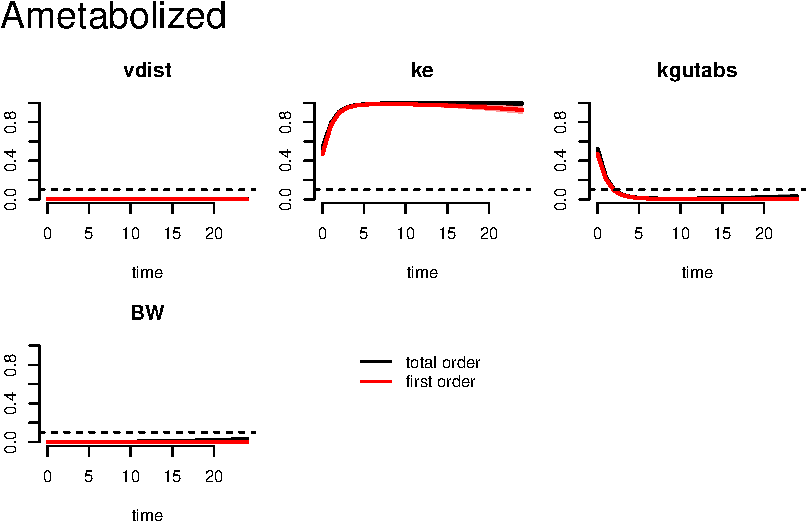
\includegraphics[width=0.8\linewidth]{RJ-pksensi_files/figure-latex/unnamed-chunk-12-1} 

}

\caption{\label{fig:pk-solvefun-Amet}Time-dependent SI of the plasma concentration estimated from the one-compartment PK model during 24-hr time period intake.}\label{fig:unnamed-chunk-12}
\end{figure}
\end{Schunk}

Figure \ref{fig:pk-solvefun-Amet} shows that the amount of metabolized
is also determined by parameter \code{ke}. Same as \code{Ccompartment},
the \code{kgutabs} contribute about 30 - 40\% variation of model output
in the first hour. The \code{BW} is the least important parameter in the
current analysis, and therefore, can be fixed in the model fitting to
data and additional applications.

In addition to using the time-SI profile to investigate the parameter
impact on model output, we can directly examine the relationship between
parameters and model output graphically.

\begin{Schunk}
\begin{Sinput}
par(mfcol=c(4,4),mar=c(0.8,0.8,0,0),oma=c(4,4,2,1), pch = ".")
plot(x$a[,1,"vdist"], out$y[,1,"0.01",1], xaxt="n", main = "\nvdist")
plot(x$a[,1,"vdist"], out$y[,1,"2.01",1], xaxt="n")
plot(x$a[,1,"vdist"], out$y[,1,"6.01",1], xaxt="n")
plot(x$a[,1,"vdist"], out$y[,1,"24.01",1])
for (j in c("ke", "kgutabs", "BW")){
  for (k in c("0.01", "2.01", "6.01", "24.01")){
    if (k == "0.01") {
      plot(x$a[,1,j], out$y[,1,k,1], yaxt = "n", xaxt="n", main = paste0("\n", j))
    } else if (k == "24.01") {
      plot(x$a[,1,j], out$y[,1,k,1], yaxt = "n")
      } else plot(x$a[,1,j], out$y[,1,k,1], xaxt = "n", yaxt = "n")
  }
}
mtext("Parameter", SOUTH<-1, line=2, outer=TRUE)
mtext("Ccompartment", WEST<-2, line=2, outer=TRUE)
\end{Sinput}
\begin{figure}

{\centering 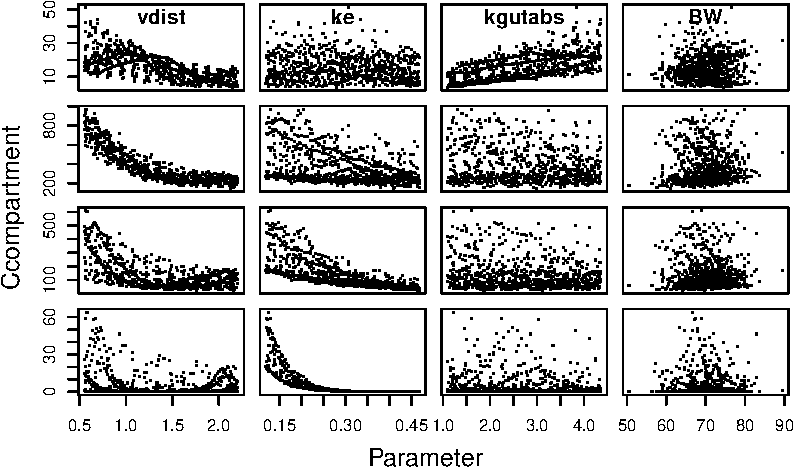
\includegraphics[width=0.95\linewidth]{RJ-pksensi_files/figure-latex/unnamed-chunk-13-1} 

}

\caption{\label{fig:SI-output}The relationship between model parameter and estimated concentration at times 0.01, 2.01, 6.01, and 24.01 hr (top to bottom), respectively.}\label{fig:unnamed-chunk-13}
\end{figure}
\end{Schunk}

Figure \ref{fig:SI-output} shows the relationship between the
concentration of the rest of the body (\code{Ccompartment}) and the
model parameters at different time points. We can find that
\code{kgutabs} and \code{vdist} have higher correlation with
\code{Ccompartment} in the beginning (t = 0.01 h) of post-intake
duration compared with other parameters, suggesting that the parameters
have high impact on the modeling result. The \code{ke} shows a high
correlation at the later time period (t = 24.01 h). The parameter
\code{BW} does not show any obvious relationship with
\code{Ccompartment}.

The output variable \code{out} containing all the input arguments
detailed above and the calculated SI of first order (\code{mSI}),
interaction (\code{iSI}), and total order (\code{tSI}). Convergence
indices are also stored in the list named \code{mCI}, \code{iCI}, and
\code{tCI}. The outputs are formatted as 4-D array in \code{y} with the
dimension name of model evaluation, number of replications, number of
time points, and number of output variables, respectively.

\begin{Schunk}
\begin{Sinput}
dim(out$y)
\end{Sinput}
\begin{Soutput}
  [1] 800  10  25   2
\end{Soutput}
\end{Schunk}

Some functions in \CRANpkg{pksensi} provide efficient ways to check the
result from global SA. The \code{check} can determine which parameters
have relatively lowered sensitivity measurement across the given time
points and model outputs, and therefore can be applied parameter fixing
in model calibration. The \code{check} also provides an argument to
specify the target output or change the cut-off value. The argument of
\code{SI.cutoff} set for example at 0.05, is used to detect the relative
non-influential parameters as default, in this case representing a 5\%
change of the output is contributed from the specific parameter
variation.

\begin{Schunk}
\begin{Sinput}
check(out, SI.cutoff = 0.05)
\end{Sinput}
\begin{Soutput}
  
  Sensitivity check ( Index > 0.05 )
  ----------------------------------
  First order:
   vdist ke kgutabs 
  
  Interaction:
   vdist ke kgutabs 
  
  Total order:
   vdist ke kgutabs 
  
  Unselected factors in total order:
   BW 
  
  
  Convergence check ( Index > 0.05 )
  ----------------------------------
  First order:
   ke kgutabs 
  
  Interaction:
   vdist 
  
  Total order:
   vdist ke
\end{Soutput}
\end{Schunk}

Based on the sensitivity measurement of the total order, the result
shows that \code{BW} has a relative lower measurement of SI. However,
all parameters do not converge to the setting cut-off, which means the
larger sample size is required in further sensitivity testing. Similar
to the \code{plot} function that can assign specific output variable in
the examination, the \code{check} function can also use the assignment
(\code{vars}) to examine a given output.

\hypertarget{model-implementation-with-gnu-mcsim}{%
\subsubsection{Model implementation with GNU
MCSim}\label{model-implementation-with-gnu-mcsim}}

In addition to using \CRANpkg{deSolve} to solve differential equations
in PK model, the GNU MCSim can also be used, and provides better
computational efficiency. To start, the users need to install GNU MCSim
and related standard C compiler to solve the ODE function. The following
script will download the one-compartment PK model from
\url{https://github.com/nanhung/pksensi/blob/master/tests/pbtk1cpt.model}.

\begin{Schunk}
\begin{Sinput}
pbtk1cpt_model()
\end{Sinput}
\end{Schunk}

The computing time of using \code{solve\_fun} in SA is estimated as,

\begin{Schunk}
\begin{Sinput}
system.time(out <- solve_fun(x, time = t, 
                             func = pbtk1cpt, initState = initState, 
                             outnames = outputs))
\end{Sinput}
\begin{Soutput}
  Starting time: 2019-10-19 11:27:54
\end{Soutput}
\begin{Soutput}
  Ending time: 2019-10-19 11:29:25
\end{Soutput}
\begin{Soutput}
     user  system elapsed 
   90.415   0.008  90.452
\end{Soutput}
\end{Schunk}

Then, before we conduct the SA through GNU MCSim, The following codes
are used to compile the GNU MCSim model code to the executable program.
To solve ODEs through GNU MCSim, we need to use \code{compile\_model}
with argument \code{application = mcsim}.

\begin{Schunk}
\begin{Sinput}
mName <- "pbtk1cpt"
compile_model(mName, application = "mcsim")
\end{Sinput}
\begin{Soutput}
  * Created executable file 'mcsim.pbtk1cpt'.
\end{Soutput}
\end{Schunk}

Similar to \code{solve\_fun} function that can define the initial values
of parameters and state variable through generated functions, the
\code{solve\_mcsim} also has a \code{condition} argument that can be
used to give the specific input value such as exposure dose, nominated
parameter value, or initial condition of state variables.

\begin{Schunk}
\begin{Sinput}
conditions <- c("Agutlument = 10") 
system.time(out <- solve_mcsim(x, mName = mName, params = params, 
                               vars = outputs, time = t, 
                               condition = conditions))
\end{Sinput}
\begin{Soutput}
  Starting time: 2019-10-19 11:29:25
\end{Soutput}
\begin{Soutput}
  * Created input file "sim.in".
\end{Soutput}
\begin{Soutput}
  Execute: ./mcsim.pbtk1cpt sim.in
\end{Soutput}
\begin{Soutput}
  Ending time: 2019-10-19 11:29:27
\end{Soutput}
\begin{Soutput}
     user  system elapsed 
    1.772   0.041   1.801
\end{Soutput}
\end{Schunk}

After solving the equations under the same given condition, we can find
that GNU MCSim has more than 10 times faster in computing performance
than using \CRANpkg{deSolve}. In this case, we only focus on performing
the global SA alone for generic PK model without additional comparison
with experimental data. The next example will display and reproduce our
previous published result \citep{fphar201800588} with full global SA
workflow.

\hypertarget{example-2-acetaminophen-pbpk-model}{%
\section{Example 2: Acetaminophen-PBPK
model}\label{example-2-acetaminophen-pbpk-model}}

This section aims to apply global SA for APAP-PBPK model through
\CRANpkg{pksensi}. The model describes the PK of parent APAP and its two
metabolites glucuronide (APAP-G) and sulfate (APAP-S). The model code is
included in this package in
\url{https://github.com/nanhung/pksensi/blob/master/tests/pbpk_apap.model}
and can generate through \code{pbpk\_apap\_model} function. We apply the
global SA workflow to the original published model with 21 model
parameters \citep{s13318-015-0253-x}. The descriptions of each parameter
and the sampling range are list in Table \ref{tab:data}.

\begin{table}[ht]
\centering
\begingroup\fontsize{8pt}{9pt}\selectfont
\begin{tabular}{lllrr}
  \hline
Parameter & Description & Unit & Min & Max \\ 
  \hline
Tg & Gatric emptying time constant & $h$ & -3.43 & 0.49 \\ 
  Tp & GI perfusion time constant & $h$ & -5.37 & -1.45 \\ 
  CYP\_Km & Cytochrome P450 metabolism, Km & $\mu{M}$ & 3.00 & 7.00 \\ 
  CYP\_VmaxC & Cytochrome P450 metabolism, VMax & $\mu{mole}/h\cdot{BW}^{0.75}$ & -1.97 & 7.97 \\ 
  SULT\_Km\_apap & Sulfation pathway acetaminophen, Km & $\mu{M}$ & 3.74 & 7.66 \\ 
  SULT\_Ki & Sulfation pathway substrate inhibition, Ki & $\mu{M}$ & 4.30 & 8.22 \\ 
  SULT\_Km\_paps & Sulfation pathway PAPS, Km & $-$ & -3.00 & 1.00 \\ 
  SULT\_VmaxC & Sulfation pathway acetaminophen, Vmax & $\mu{mole}/h\cdot{BW}^{0.75}$ & 0.00 & 10.00 \\ 
  UGT\_Km & Glucuronidation pathway acetaminophen, Km & $\mu{M}$ & 6.74 & 10.66 \\ 
  UGT\_Ki & Glucuronidation pathway substrate inhibition, Ki & $\mu{M}$ & 9.01 & 12.93 \\ 
  UGT\_Km\_GA & Glucuronidation pathway GA, Km & $-$ & -3.00 & 1.00 \\ 
  UGT\_VmaxC & Glucuronidation pathway acetaminophen, Vmax & $\mu{mole}/h\cdot{BW}^{0.75}$ & 0.00 & 10.00 \\ 
  Km\_AG & APAP-G hepatic transporter, Km & $\mu{M}$ & 7.94 & 11.86 \\ 
  Vmax\_AG & APAP-G hepatic transporter, Vmax & $\mu{mole}/h$ & 6.99 & 15.00 \\ 
  Km\_AS & APAP-S hepatic transporter, Km & $\mu{M}$ & 8.00 & 12.00 \\ 
  Vmax\_AS & APAP-S hepatic transporter, Vmax & $\mu{mole}/h$ & 6.99 & 15.00 \\ 
  kGA\_syn & UDPGA synthesis & $1/h$ & 0.00 & 13.00 \\ 
  PAPS\_syn & PAPS synthesis & $1/h$ & 0.00 & 13.00 \\ 
  CLC\_APAP & APAP clearance & $L/h\cdot{BW}^{0.75}$ & -6.00 & 1.00 \\ 
  CLC\_AG & APAP-G clearance & $L/h\cdot{BW}^{0.75}$ & -6.00 & 1.00 \\ 
  CLC\_AS & APAP-S clearance & $L/h\cdot{BW}^{0.75}$ & -6.00 & 1.00 \\ 
   \hline
\end{tabular}
\endgroup
\caption{\label{tab:data}Description of sampling range of model parameter.} 
\end{table}

As in the example of the one-compartment PK model, the model parameter
and the corresponding sampling range should be defined to create the
parameter matrix. Previously, the probability distributions of model
parameters were set to either truncated normal or uniform distributions
when the parameters have informative prior information or not,
respectively. To rapidly reach the acceptable convergence in this
example, we use a uniform distribution for all testing parameters. The
ranges of informative parameters set to 1.96-times difference for the
single side under log-scaled (approximate 54.6 times difference between
minimum and maximum in natural scaled). The nominal values of
informative model parameters define as:

\begin{Schunk}
\begin{Sinput}
Tg <- log(0.23)
Tp <- log(0.033)
CYP_Km <- log(130)
SULT_Km_apap <- log(300)
SULT_Ki <- log(526)
SULT_Km_paps <- log(0.5)
UGT_Km <- log(6.0e3)
UGT_Ki <- log(5.8e4)
UGT_Km_GA <-log(0.5)
Km_AG <- log(1.99e4)
Km_AS <- log(2.29e4)
rng <- 1.96 
\end{Sinput}
\end{Schunk}

Generally, a wide range of parameter value might cause the computing
error when solving the differential equation. One of the effective ways
to prevent this problem is to adjust the value of relative and absolute
error tolerance to control the error appearance by resetting these
parameters in the lower levels. The \code{generate\_infile} and
\code{solve\_mcsim} functions provide arguments of \code{rtol} and
\code{atol} that adjust the error tolerance to prevent the unwanted
error. However, the modification will decrease the computing speed.
Therefore, the alternative method to prevent this issue is to detect the
crucial parameter range that causes the problem. Also, setting the
maximum number of steps to the higher value in GNU MCSim can prevent
this problem (internally defined). The maximum number of step is 5000
(default) in this case. The value can reset through reinstallation of
GNU MCSim. Here we separate the global SA of APAP-PBPK model process to
several steps.

\hypertarget{prepare-and-compile-the-model-file}{%
\subsection{Prepare and compile the model
file}\label{prepare-and-compile-the-model-file}}

The model code needs to prepare in the following global SA workflow.
After creating the \code{pbpk\_apap.model} file in the working
directory, the next step is to generate the executable program
(\code{mcsim.pbpk\_apap}) through the \code{compile\_model} function.

\begin{Schunk}
\begin{Sinput}
mName <- "pbpk_apap"
pbpk_apap_model()
compile_model(mName, application = "mcsim")
\end{Sinput}
\begin{Soutput}
  * Created executable file 'mcsim.pbpk_apap'.
\end{Soutput}
\end{Schunk}

\hypertarget{define-the-parameter-and-its-distribution}{%
\subsection{Define the parameter and its
distribution}\label{define-the-parameter-and-its-distribution}}

The 21 tested model parameters are defined in this step, including
parameter names and probability distributions. To prevent errors, the
ranges of \code{SULT\_VmaxC} and \code{UGT\_VmaxC} need to be adjusted
from \(U(0, 15)\) \citep{s13318-015-0253-x} to \(U(0, 10)\)
\citep{fphar201800588}. The objects \code{q} and \code{dist} are set to
the type of distribution that will be used to generate the parameter
matrix in GNU MCSim (for uncertainty analysis) and R (for SA).

\begin{Schunk}
\begin{Sinput}
params <- c("lnTg", "lnTp", "lnCYP_Km","lnCYP_VmaxC",
           "lnSULT_Km_apap","lnSULT_Ki","lnSULT_Km_paps","lnSULT_VmaxC",
           "lnUGT_Km","lnUGT_Ki","lnUGT_Km_GA","lnUGT_VmaxC",
           "lnKm_AG","lnVmax_AG","lnKm_AS","lnVmax_AS",
           "lnkGA_syn","lnkPAPS_syn", "lnCLC_APAP","lnCLC_AG","lnCLC_AS")
dist <- rep("Uniform", 21)
q <- rep("qunif", 21)
q.arg <-list(list(Tg-rng, Tg+rng), list(Tp-rng, Tp+rng), 
             list(CYP_Km-rng, CYP_Km+rng), list(-2., 5.),
             list(SULT_Km_apap-rng, SULT_Km_apap+rng),
             list(SULT_Ki-rng, SULT_Ki+rng),
             list(SULT_Km_paps-rng, SULT_Km_paps+rng),
             list(0, 10), list(UGT_Km-rng, UGT_Km+rng),
             list(UGT_Ki-rng, UGT_Ki+rng),
             list(UGT_Km_GA-rng, UGT_Km_GA+rng),
             list(0, 10), list(Km_AG-rng, Km_AG+rng),
             list(7., 15), list(Km_AS-rng, Km_AS+rng),
             list(7., 15), list(0., 13), list(0., 13),
             list(-6., 1), list(-6., 1), list(-6., 1))
\end{Sinput}
\end{Schunk}

\hypertarget{define-additional-input-condition-and-output-time-and-variables}{%
\subsection{Define additional input condition and output time and
variables}\label{define-additional-input-condition-and-output-time-and-variables}}

In this case, we only use GNU MCSim to estimate the concentration of
APAP and its metabolites in plasma to optimize the computing speed. The
oral dose of APAP is 20 mg/kg in this example. Generally, the input
dosing method can be defined through the \code{condition} argument.
Since the unit of the given dose is mg/kg, the \code{mgkg\_flag} is set
to 1. Additional input schedule functions can be found in the section of
input functions in GNU MCSim User's Manual
(\url{https://www.gnu.org/software/mcsim/mcsim.html\#Input-functions}).

\begin{Schunk}
\begin{Sinput}
conditions <- c("mgkg_flag = 1",
                "OralExp_APAP = NDoses(2, 1, 0, 0, 0.001)",
                "OralDose_APAP_mgkg = 20.0")
vars <- c("lnCPL_APAP_mcgL", "lnCPL_AG_mcgL", "lnCPL_AS_mcgL")
times <- seq(from = 0.1, to = 12.1, by = 0.2)
\end{Sinput}
\end{Schunk}

\hypertarget{uncertainty-analysis}{%
\subsubsection{Uncertainty analysis}\label{uncertainty-analysis}}

We apply uncertainty analysis through the \code{solve\_mcsim} function
and visualize the results using \code{pksim} function. Some example data
are included in \CRANpkg{pksensi} with experiment time (h) and
concentration (mg/L).

\begin{Schunk}
\begin{Sinput}
head(APAP)
\end{Sinput}
\begin{Soutput}
    Wt Time APAP    AG   AS         Study Dose
  1 72 0.25 15.5  3.20 3.55 Prescott_1980   20
  2 72 0.50 18.7  7.95 6.75 Prescott_1980   20
  3 72 0.75 18.8 13.42 8.21 Prescott_1980   20
  4 72 1.00 18.0 18.14 9.56 Prescott_1980   20
  5 72 1.50 15.6 24.68 9.35 Prescott_1980   20
  6 72 2.00 13.6 27.28 8.78 Prescott_1980   20
\end{Soutput}
\end{Schunk}

In setting simulation conditions, the relative and absolute error
tolerance (\code{rtol} \& \code{atol}) were set to 1e-7 and 1e-9,
respectively, to prevent the numerical errors. The Monte Carlo
simulation is run for 1000 iterations in the assignment of
\code{monte\_carlo}. The input file (\texttt{sim.in}) and output file
(\texttt{simmc.out}) will be generated under the standard ASCII format.

\begin{Schunk}
\begin{Sinput}
set.seed(1111)
out <- solve_mcsim(mName = mName, params = params, vars = vars,
                   monte_carlo = 1000, dist = dist, q.arg = q.arg, 
                   time = times, condition = conditions, 
                   rtol = 1e-7, atol = 1e-9)
\end{Sinput}
\begin{Soutput}
  Starting time: 2019-10-19 11:29:28
\end{Soutput}
\begin{Soutput}
  * Created input file "sim.in".
\end{Soutput}
\begin{Soutput}
  Execute: ./mcsim.pbpk_apap sim.in
\end{Soutput}
\begin{Soutput}
  Ending time: 2019-10-19 11:29:30
\end{Soutput}
\end{Schunk}

Figure \ref{fig:pksim-MC} shows the uncertainty analysis of APAP data
and modeling results. For parent compound, all data points are located
in the simulated interval of 25-75\%, suggesting that the simulated
outputs can accurately cover the experimental concentration profiles
under the assumed parameter ranges for APAP. The simulated results of
metabolites APAP-G and APAP-S, while not fully in the 25-75\% range, and
nonetheless within the envelope of the simulated intervals.

\begin{Schunk}
\begin{Sinput}
par(mfrow = c(1,3), mar = c(4,4,1,1))
pksim(out, xlab = "Time (h)", ylab = "Conc. (ug/L)", main = "APAP")
points(APAP$Time, log(APAP$APAP * 1000))
pksim(out, vars = "lnCPL_AG_mcgL", xlab = "Time (h)", main = "APAP-G", 
      ylab = " ", legend = FALSE)
points(APAP$Time, log(APAP$AG * 1000))
pksim(out, vars = "lnCPL_AS_mcgL", xlab = "Time (h)", main = "APAP-S", 
      ylab = " ", legend = FALSE)
points(APAP$Time, log(APAP$AS * 1000))
\end{Sinput}
\begin{figure}

{\centering 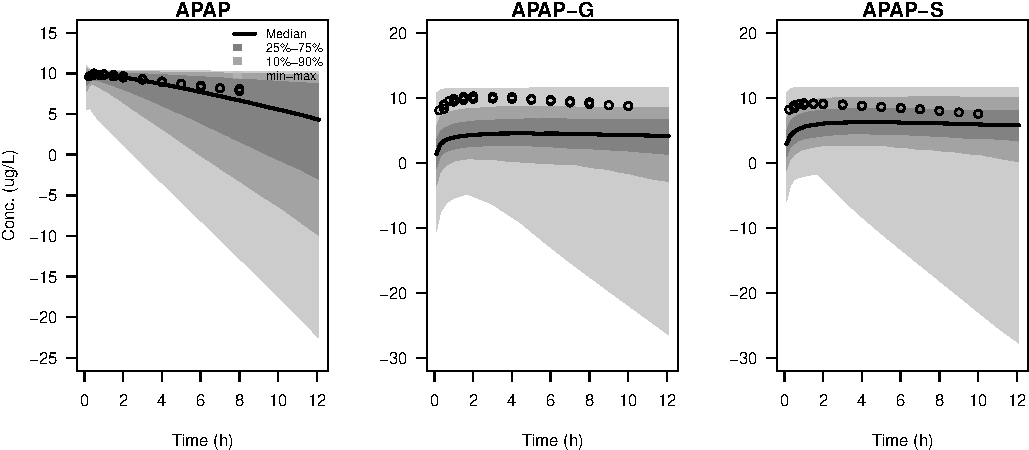
\includegraphics[width=1\linewidth]{RJ-pksensi_files/figure-latex/unnamed-chunk-27-1} 

}

\caption{\label{fig:pksim-MC}Coverage checks of prior PBPK model predictions with calibrated APAP data.}\label{fig:unnamed-chunk-27}
\end{figure}
\end{Schunk}

\hypertarget{generate-parameter-matrix}{%
\subsubsection{Generate parameter
matrix}\label{generate-parameter-matrix}}

To perform global SA, we next have to generate the parameter matrix from
the eFAST method. An example with sample size 512 with 10 replications
would be as follows:

\begin{Schunk}
\begin{Sinput}
set.seed(1234)
x <- rfast99(params = params, n = 512, q = q, q.arg = q.arg, replicate = 10) 
\end{Sinput}
\end{Schunk}

\hypertarget{conduct-the-global-sa}{%
\subsubsection{Conduct the global SA}\label{conduct-the-global-sa}}

To conduct the global SA with GNU MCSim and \CRANpkg{pksensi}, an input
file needs to be generate before modeling. The file can be created by
the \code{generate\_infile} function. Alternatively, \code{solve\_mcsim}
can also automatically create the input file and compute the output.

\begin{Schunk}
\begin{Sinput}
out <- solve_mcsim(x, mName = mName,
                   params = params, 
                   time = times, 
                   vars = vars,
                   condition = conditions, 
                   rtol = 1e-7, atol = 1e-9)
\end{Sinput}
\begin{Soutput}
  Starting time: 2019-10-19 11:29:31
\end{Soutput}
\begin{Soutput}
  * Created input file "sim.in".
\end{Soutput}
\begin{Soutput}
  Execute: ./mcsim.pbpk_apap sim.in
\end{Soutput}
\begin{Soutput}
  Ending time: 2019-10-19 11:33:25
\end{Soutput}
\end{Schunk}

\hypertarget{visualization-and-decision}{%
\subsubsection{Visualization and
decision}\label{visualization-and-decision}}

The plotting function can show the results of time-dependent sensitivity
to determine the parameter impacts on model output over time (Figure
\ref{fig:APAP-sensi}).

\begin{Schunk}
\begin{Sinput}
plot(out, vars = "lnCPL_APAP_mcgL")
\end{Sinput}
\begin{figure}

{\centering 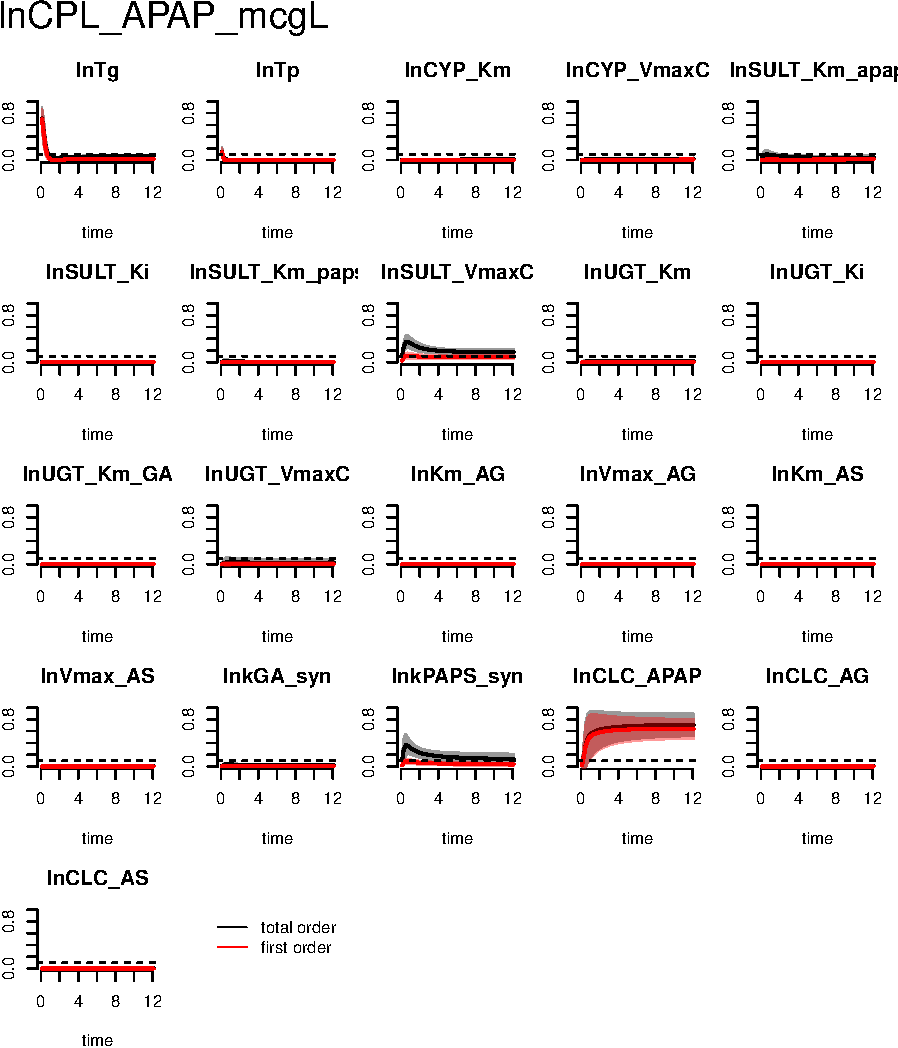
\includegraphics[width=0.8\linewidth]{RJ-pksensi_files/figure-latex/unnamed-chunk-30-1} 

}

\caption{\label{fig:APAP-sensi}Time-dependent SI of the plasma APAP concentration estimated from APAP-PBPK model during 12-hr time period post intake.}\label{fig:unnamed-chunk-30}
\end{figure}
\end{Schunk}

Based on our previous study, we propose the heatmap visualization
approach \code{heat\_check} to distinguish ``influential'' and
``non-influential'' parameters with a ``cut-off'' point. Through the
given argument \code{order}, we can select the specific order of
sensitivity measurement that we are interested in (Figure
\ref{fig:Heat-SI}).

\begin{Schunk}
\begin{Sinput}
heat_check(out, order = "total order")
\end{Sinput}
\begin{figure}

{\centering 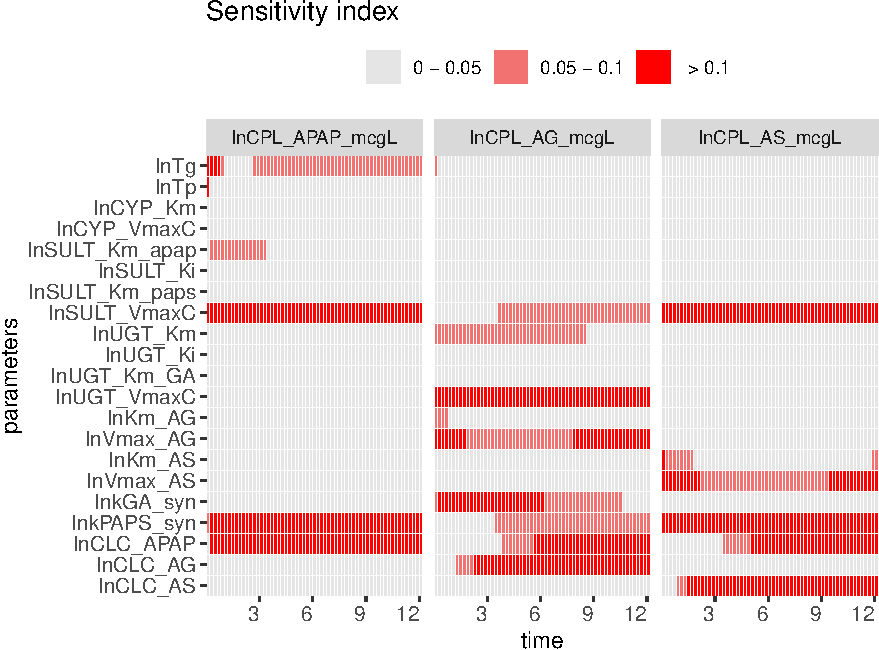
\includegraphics[width=0.8\linewidth]{RJ-pksensi_files/figure-latex/unnamed-chunk-31-1} 

}

\caption{\label{fig:Heat-SI}Heat map representation of time-dependent total SI computed in global SA method.}\label{fig:unnamed-chunk-31}
\end{figure}
\end{Schunk}

Adding the \texttt{index\ =\ "CI"} in the function can further
investigate the convergence index. Based on the current setting of
sampling size, most parameters cannot reach the acceptable criteria of
convergence (Figure \ref{fig:Heat-CI}). Therefore, a higher number of
sampling is necessary. The sample size of convergence in the current
PBPK model is 8,192 \citep{fphar201800588}. However, based on the
current sample size, we still can find 6 parameters that can be an
important parameter for the plasma APAP concentration.

\begin{Schunk}
\begin{Sinput}
heat_check(out, index = "CI", order = "total order")
\end{Sinput}
\begin{figure}

{\centering 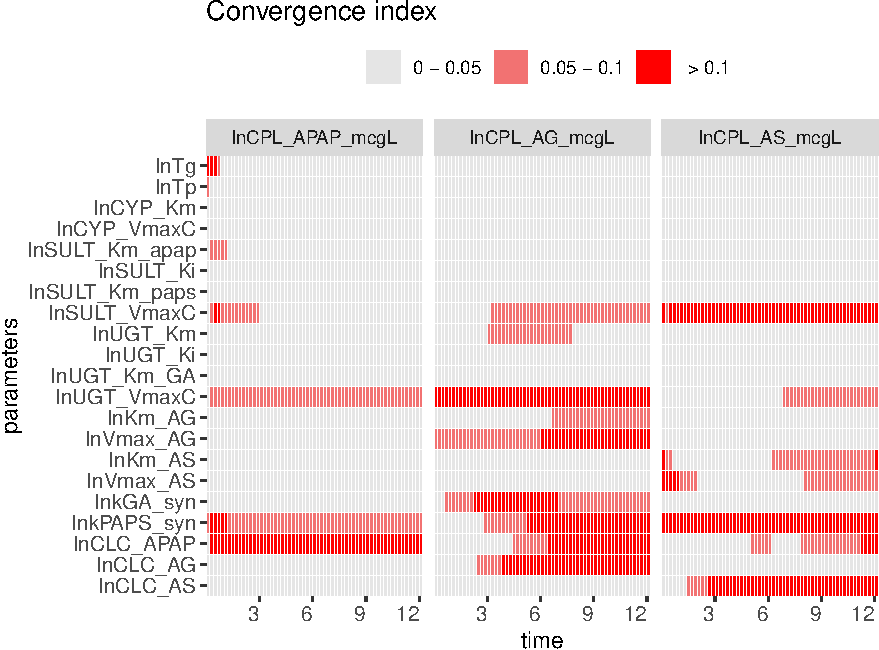
\includegraphics[width=0.8\linewidth]{RJ-pksensi_files/figure-latex/unnamed-chunk-32-1} 

}

\caption{\label{fig:Heat-CI}Heat map representation of time-dependent total CI computed in global SA method.}\label{fig:unnamed-chunk-32}
\end{figure}
\end{Schunk}

\hypertarget{conclusions-and-perspectives}{%
\section{Conclusions and
perspectives}\label{conclusions-and-perspectives}}

We initiated \CRANpkg{pksensi} in order to facilitate a comprehensive
and efficient global SA workflow in PK modeling, filling a crucial gap
for open-source modeling communities. It provides a straightforward
application to investigate the impact of parameters on model outputs
across simulation time-points and variables. We adopted the eFAST
method, a common variance-based SA that we found to have the best
balance of efficiency and accuracy. In addition, the package also
includes the ability to assess the convergence of SA results, which is
rarely addressed in most global SA studies and software packages. We
also developed functions to visualize the output results and help
distinguish the ``influential'' and ``non-influential'' parameters that
can be applied in parameter fixing in the model calibration. In future
versions, we expect to add additional global SA approaches
\citep{glen2012estimating, ring2017identifying}. Other features, such as
principle component analysis \citep{lamboni2011multivariate} will also
be considered.

We chose to integrate sensitivity analysis with GNU MCSim because it is
a powerful open-source software package for dynamical simulation of
biological-based models, mainly built for PK research with probabilistic
approaches \citep{bois2009gnu}. In addition, the current version of
\CRANpkg{pksensi} includes both GNU MCSim and \CRANpkg{deSolve} as the
main ODE solvers. Compared with the \CRANpkg{deSolve} package, the GNU
MCSim can provide better speed and efficiency to solve the ODEs in PK
models. Although \CRANpkg{pksensi} provides the essential features and
functions to install and link with GNU MCSim, conducting the uncertainty
and SA in PK modeling, the overall learning curve of this workflow might
steep for users that are not familiar with GNU MCSim from model
development, debugging, and testing. Therefore, the general package,
such as \CRANpkg{deSolve}, can be an alternative option for R users.
Some other packages are also available to solve ODEs, such as
\CRANpkg{RxODE} \citep{wang2016tutorial} and \CRANpkg{mrgsolve}
\citep{R-mrgsolve}. We hope to incorporate these packages to expand the
flexibility of using \CRANpkg{pksensi} in the future. It addition,
\CRANpkg{pksensi} also has potential to be performed in interactive PBPK
modeling platform \citep{li2019integration}.

It is worth noting that the current global SA results are conditional on
the specific model and the given range of the model parameters. Other
factors, such as the number of parameters examined, the parameter
distributions/ranges, and the given dosing level in PK model might also
have a potential impact on the level of importance of each parameter,
but these ``meta-uncertainties'' are not currently addressed. Complex
models with high paremeter dimensionality are also challenging in global
SA as they have higher computer demands. As approaches are developed to
address these complexities, we hope to incorporate them into
\CRANpkg{pksensi}.

Overall, \CRANpkg{pksensi} provides comprehensive suite of features and
functions for performing global SA for PK models and can create robust
and reproducible results for decision making in model development and
calibration. Although \CRANpkg{pksensi} used here is mainly for PK
modeling, it can also be applied to other ODE-based dynamic models in
order to investigate the sensitivity of model outputs to input
parameters.

\hypertarget{code}{%
\subsection{Code}\label{code}}

The source material for this paper is available at
\url{https://github.com/nanhung/RJ-pksensi}.

\hypertarget{acknowledgments}{%
\subsection{Acknowledgments}\label{acknowledgments}}

This work was funded, in part, by grant 1U01FD005838 from the U.S. Food
and Drug Administration (FDA) and grant P42 ES027704 from the U.S.
National Institute of Environmental Health Sciences. This article
reflects the views of the author and should not be construed to
represent FDA's views or policies. We thank Dr.~Yasha Hartberg and
Dr.~Barbara Gastel at the Texas A\&M University, Dr.~Frederic Bois from
Certara and Dr.~Eleftheria Tsakalozou from U.S. FDA for reviewing the
manuscript and consultation.

\hypertarget{session-information}{%
\section{Session information}\label{session-information}}

\begin{itemize}\raggedright
  \item R version 3.6.1 (2019-07-05), \verb|x86_64-pc-linux-gnu|
  \item Locale: \verb|LC_CTYPE=en_US.UTF-8|, \verb|LC_NUMERIC=C|, \verb|LC_TIME=en_US.UTF-8|, \verb|LC_COLLATE=en_US.UTF-8|, \verb|LC_MONETARY=en_US.UTF-8|, \verb|LC_MESSAGES=en_US.UTF-8|, \verb|LC_PAPER=en_US.UTF-8|, \verb|LC_NAME=C|, \verb|LC_ADDRESS=C|, \verb|LC_TELEPHONE=C|, \verb|LC_MEASUREMENT=en_US.UTF-8|, \verb|LC_IDENTIFICATION=C|
  \item Running under: \verb|elementary OS 5.0 Juno|
  \item Matrix products: default
  \item BLAS:   \verb|/usr/lib/x86_64-linux-gnu/openblas/libblas.so.3|
  \item LAPACK: \verb|/usr/lib/x86_64-linux-gnu/libopenblasp-r0.2.20.so|
  \item Base packages: base, datasets, graphics, grDevices,
    methods, stats, utils
  \item Other packages: deSolve~1.24, httk~1.10.0,
    pksensi~1.1.3.9000, xtable~1.8-4
  \item Loaded via a namespace (and not attached):
    assertthat~0.2.1, colorspace~1.4-1, compiler~3.6.1,
    crayon~1.3.4, data.table~1.12.2, DBI~1.0.0, digest~0.6.20,
    dplyr~0.8.3, evaluate~0.14, expm~0.999-4, getPass~0.2-2,
    ggplot2~3.2.1, glue~1.3.1, grid~3.6.1, gtable~0.3.0,
    htmltools~0.3.6, knitr~1.25, labeling~0.3, lattice~0.20-38,
    lazyeval~0.2.2, magrittr~1.5, Matrix~1.2-17, mitools~2.4,
    msm~1.6.7, munsell~0.5.0, mvtnorm~1.0-11, pillar~1.4.2,
    pkgconfig~2.0.2, plyr~1.8.4, purrr~0.3.2, R6~2.4.0,
    Rcpp~1.0.2, reshape~0.8.8, reshape2~1.4.3, rlang~0.4.0,
    rmarkdown~1.15, rticles~0.10, scales~1.0.0, splines~3.6.1,
    stringi~1.4.3, stringr~1.4.0, survey~3.36, survival~2.44-1.1,
    tibble~2.1.3, tidyselect~0.2.5, tools~3.6.1, xfun~0.9,
    yaml~2.2.0
\end{itemize}

\bibliography{RJreferences}


\address{%
Nan-Hung Hsieh\\
Veterinary Integrative Biosciences, College of Veterinary Medicine and
Biomedical Sciences, Texas A\&M University\\
College Station, TX, USA\\
}
\href{mailto:nhsieh@cvm.tamu.edu}{\nolinkurl{nhsieh@cvm.tamu.edu}}

\address{%
Brad Reisfeld\\
Chemical and Biological Engineering and School of Biomedical
Engineering, Colorado State University\\
Fort Collins, CO, USA\\
}
\href{mailto:brad.reisfeld@colostate.edu}{\nolinkurl{brad.reisfeld@colostate.edu}}

\address{%
Weihsueh A. Chiu\\
Veterinary Integrative Biosciences, College of Veterinary Medicine and
Biomedical Sciences, Texas A\&M University\\
College Station, TX, USA\\
}
\href{mailto:wchiu@cvm.tamu.edu}{\nolinkurl{wchiu@cvm.tamu.edu}}

